\documentclass[dvipsnames, tikz]{standalone}
\usepackage{amsmath}
\usepackage{arevmath}
\usepackage{xcolor}
\usepackage{tikz}
\usetikzlibrary{calc}
\usetikzlibrary{decorations.pathreplacing,calligraphy,3d}
\usetikzlibrary{matrix,shapes,fit,backgrounds}


\begin{document}
	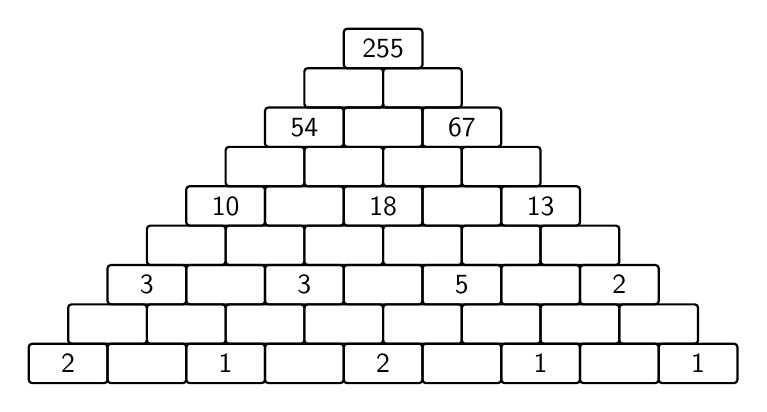
\begin{tikzpicture}[color=black, font=\sf]
		\foreach \x in {0,...,8}{
			\foreach \y in  {0,...,\x}{
				\draw[thick, rounded corners=1.2pt] (-0.5-0.5*\x+\y, -0.25-\x/2) rectangle ++(1,0.5);
			}
		}
		\draw (0,0) node {255};
		
		\draw (-1,-1) node {54};
		\draw (1,-1) node {67};
		
		\draw (-2,-2) node {10};
		\draw (0,-2) node {18};
		\draw (2,-2) node {13};
		
		\draw (-3,-3) node {3};
		\draw (-1,-3) node {3};
		\draw (1,-3) node {5};
		\draw (3,-3) node {2};
		
		\draw (-4,-4) node {2};
		\draw (-2,-4) node {1};
		\draw (0,-4) node {2};
		\draw (2,-4) node {1};
		\draw (4,-4) node {1};
	\end{tikzpicture}
\end{document}